% ------------------------------------------------------------------------
% ------------------------------------------------------------------------
% Modelo UFSC para Trabalhos Academicos (tese de doutorado, dissertação de
% mestrado) utilizando a classe abntex2
%
% Autor: Alisson Lopes Furlani
% 	Modificações:
%	- 27/08/2019: Alisson L. Furlani, add pacote 'glossaries' para listas
%   - 06/11/2019: Luiz-Rafael Santos, modifica para Trabalho de Conclusão de Curso
% ------------------------------------------------------------------------
% ------------------------------------------------------------------------

\documentclass[
	% -- opções da classe memoir --
	12pt,				% tamanho da fonte
	%openright,			% capítulos começam em pág ímpar (insere página vazia caso preciso)
	oneside,			% para impressão no anverso. Oposto a twoside
	a4paper,			% tamanho do papel. 
	% -- opções da classe abntex2 --
	chapter=TITLE,		% títulos de capítulos convertidos em letras maiúsculas
	section=TITLE,		% títulos de seções convertidos em letras maiúsculas
	%subsection=TITLE,	% títulos de subseções convertidos em letras maiúsculas
	%subsubsection=TITLE,% títulos de subsubseções convertidos em letras maiúsculas
	% -- opções do pacote babel --
	english,			% idioma adicional para hifenização
	%french,				% idioma adicional para hifenização
	%spanish,			% idioma adicional para hifenização
	brazil				% o último idioma é o principal do documento
	]{abntex2}

\usepackage{setup/ufscthesisA4-alf}
\usepackage{siunitx}
\usepackage{array} % for the 'p' column type
\usepackage{multirow}
\usepackage{lscape}
\usepackage{float}
\usepackage{hyperref}
% \usepackage{graphicx}

% ---
% Filtering and Mapping Bibliographies
% ---
% Pacotes de citações
% ---
\usepackage{csquotes}
\usepackage[backend = biber, style = abnt]{biblatex}
% FIXME Se desejar estilo numérico de citações,  comente a linha acima e descomente a linha a seguir.
% \usepackage[backend = biber, style = numeric-comp]{biblatex}

\setlength\bibitemsep{\baselineskip}
\DeclareFieldFormat{url}{Disponível~em:\addspace\url{#1}}
\NewBibliographyString{sineloco}
\NewBibliographyString{sinenomine}
\DefineBibliographyStrings{brazil}{%
	sineloco     = {\mkbibemph{S\adddot l\adddot}},
	sinenomine   = {\mkbibemph{s\adddot n\adddot}},
	andothers    = {\mkbibemph{et\addabbrvspace al\adddot}},
	in			 = {\mkbibemph{In:}}
}

\addbibresource{aftertext/references.bib} % Seus arquivos de referências

% ---
\DeclareSourcemap{
	\maps[datatype=bibtex]{
		% remove fields that are always useless
		\map{
			\step[fieldset=abstract, null]
			\step[fieldset=pagetotal, null]
		}
		% remove URLs for types that are primarily printed
%		\map{
%			\pernottype{software}
%			\pernottype{online}
%			\pernottype{report}
%			\pernottype{techreport}
%			\pernottype{standard}
%			\pernottype{manual}
%			\pernottype{misc}
%			\step[fieldset=url, null]
%			\step[fieldset=urldate, null]
%		}
		\map{
			\pertype{inproceedings}
			% remove mostly redundant conference information
			\step[fieldset=venue, null]
			\step[fieldset=eventdate, null]
			\step[fieldset=eventtitle, null]
			% do not show ISBN for proceedings
			\step[fieldset=isbn, null]
			% Citavi bug
			\step[fieldset=volume, null]
		}
	}
}
% ---

% ---
% Informações de dados para CAPA e FOLHA DE ROSTO
% ---
% FIXME Substituir 'Nome completo do autor' pelo seu nome.
\autor{Thiago Boimer Correia}
% FIXME Substituir 'Título do trabalho' pelo título da trabalho.
\titulo{Desenvolvimento de aplicativo para cruzamento de dados entre geradores e potenciais consumidores de resíduos sólidos no Estado de Santa Catarina}
% FIXME Substituir 'Subtítulo (se houver)' pelo subtítulo da trabalho.  
% Caso não tenha substítulo, comente a linha a seguir.
% \subtitulo{um sistema de match entre indústrias}
% FIXME Substituir 'XXXXXX' pelo nome do seu
% orientador.
\orientador{Prof. Dachamir Hotza, Dr.}
% FIXME Se for orientado por uma mulher, comente a linha acima e descomente a linha a seguir.
% \orientador[Orientadora]{Nome da orientadora, Dra.}
% FIXME Substituir 'XXXXXX' pelo nome do seu
% coorientador. Caso não tenha coorientador, comente a linha a seguir.
% \coorientador{Prof. XXXXXX, Dr.}
% FIXME Se for coorientado por uma mulher, comente a linha acima e descomente a linha a seguir.
% \coorientador[Coorientadora]{XXXXXX, Dra.}
% FIXME Substituir 'XXXXXX' pelo nome do Coordenador do 
% programa/curso.
\coordenador{Prof. Celso Peres Fernandes, Dr.}
% FIXME Se for coordenadora mulher, comente a linha acima e descomente a linha a seguir.
% \coordenador[Coordenadora]{Nome da Coordenadora, Dra.}
% FIXME Substituir '[ano da entrega]' pelo ano (ano) em que seu trabalho foi defendido.
\ano{2023}
% FIXME Substituir '[dia] de [mês] de [ano]' pela data em que ocorreu sua defesa.
\data{15 de Dezembro de 2023}
% FIXME Substituir '[Cidade da defesa]' pela cidade em que ocorreu sua defesa.
\local{Florianópolis}
\instituicaosigla{UFSC}
\instituicao{Universidade Federal de Santa Catarina}
% FIXME Substituir 'Dissertação/Tese' pelo tipo de trabalho (Tese, Dissertação). 
\tipotrabalho{Trabalho de Conclusão de Curso}
% FIXME Substituir '[licenciado/bacharel] em [nome do título obtido]' pela grau adequado.
\formacao{Bacharel em Engenharia de Materiais}
% FIXME Substituir '[licenciado/bacharel]' pelo nivel adequado.
\nivel{Bacharel}
% FIXME Substituir 'Curso de Graduação em [XXXXXXXX]' pela curso adequado.
\programa{Curso de Graduação em Engenharia de Materiais}
% FIXME Substituir 'Campus XXXXXX ou Centro de XXXXXX' pelo campus ou centro adequado.
\centro{Centro Tecnológico}
\departamento{Departamento de Engenharia Mecânica e Materiais}
\preambulo
{%
\imprimirtipotrabalho~do~\imprimirprograma~do~\imprimircentro~da~\imprimirinstituicao~para~a~obtenção~do~título~de~\imprimirformacao.
}
% ---

% ---
% Configurações de aparência do PDF final
% ---
% alterando o aspecto da cor azul
\definecolor{blue}{RGB}{41,5,195}
% informações do PDF
\makeatletter
\hypersetup{
     	%pagebackref=true,
		pdftitle={\@title}, 
		pdfauthor={\@author},
    	pdfsubject={\imprimirpreambulo},
	    pdfcreator={LaTeX with abnTeX2},
		pdfkeywords={ufsc, latex, abntex2}, 
		colorlinks=true,       		% false: boxed links; true: colored links
    	linkcolor=black,%blue,          	% color of internal links
    	citecolor=black,%blue,        		% color of links to bibliography
    	filecolor=black,%magenta,      		% color of file links
		urlcolor=black,%blue,
		bookmarksdepth=4
}
\makeatother
% ---

% ---
% compila a lista de abreviaturas e siglas e a lista de símbolos
% ---

% Declaração das siglas
\siglalista{ABNT}{Associação Brasileira de Normas Técnicas}
\siglalista{NBR}{Norma Brasileira}
\siglalista{PNRS}{Política Nacional de Resíduos Sólidos}
\siglalista{RSU}{Resíduos Sólidos Urbanos}
\siglalista{RSI}{Resíduos Sólidos Industriais}
\siglalista{SC}{Santa Catarina}
\siglalista{ODS}{Objetivos de Desenvolvimento Sustentável}
\siglalista{ONU}{Organização das Nações Unidas}
\siglalista{MTR}{Manifesto de Transporte de Resíduos}
\siglalista{IMA/SC}{Instituto do Meio Ambiente de Santa Catarina}
\siglalista{IMA}{Instituto do Meio Ambiente}
\siglalista{UF}{Unidade Federativa}
\siglalista{SINIR}{Sistema Nacional de Informações Sobre a Gestão dos Resíduos Sólidos}
\siglalista{PGRS}{Plano de Gestão do dos Resíduos Sólidos}
\siglalista{OLUC}{Óleo Lubrificante Usado ou Contaminado}
\siglalista{ETE}{Estação de Tratamento de Esgoto}
\siglalista{ABETRE}{Associação Brasileira de Empresas de Tratamento de Resíduos e Efluentes}
\siglalista{IBAMA}{Instituto Brasileiro do Meio Ambiente e dos Recursos Naturais Renováveis}
\siglalista{IBGE}{Instituto Brasileiro de Geografia e Estatistica}
\siglalista{PIA}{Pesquisa Industrial Anual}
\siglalista{VTI}{Valor da Transformação Industrial}
\siglalista{CNAE}{Classificação Nacional de Atividades Econômicas}
\siglalista{RAPP}{Relatório Anual de Atividades Potencialmente Poluidoras e Utilizadoras de Recursos Ambientais}
\siglalista{MMA}{Ministério do Meio Ambiente e Mudança do Clima}
\siglalista{CPF}{Cadastro de Pessoa Física}
\siglalista{CNPJ}{Cadastro Nacional de Pessoa Jurídica}
\siglalista{CTF/APP}{Cadastro Técnico Federal de Atividades Potencialmente Poluidoras e Utilizadoras de Recursos Naturais}
\siglalista{SNIS}{Sistema Nacional de Saneamento Básico}
\siglalista{CSV}{Valores Separados por Vírgula (Comma-separated values)}
\siglalista{JSON}{Objeto de Notação de Javascript (JavaScript Object Notation)}
\siglalista{PDF}{Documento de Formato Portátil (Portable Document Format)}
\siglalista{API}{Interface de Programação de Aplicação (Application Programming Interface)}
\siglalista{URI}{Identificador Uniforme de Recurso (Uniform Resource Identifier)}
\siglalista{HTTP}{Protocolo de Transferência de Hipertexto (HyperText Transfer Protocol)}
\siglalista{CAPTCHA}{Teste de Turing Público Completamente Automatizado para distinguir entre Computadores e Pessoas (Completely Automated Public Turing test to tell Computers and Humans Apart)}
\siglalista{RAM}{Memória de Acesso Aleatório (Random Access Memory)}
\siglalista{SSD}{Unidade de Estado Sólido (Solid State Drive)}
\siglalista{SQL}{Linguagem de Consulta Estruturada (Structured Query Language)}
\siglalista{HTML}{Linguagem de Marcação de HiperTexto (Hyper Text Markup Language)}
\siglalista{CSS}{Folhas de Estilo em Cascata (Cascading Style Sheets)}
\siglalista{SSL}{Secure Sockets Layer}
\siglalista{UFSC}{Universidade Federal de Santa Catarina}
\siglalista{CETESB}{Companhia Ambiental do Estado de São Paulo}
\siglalista{IA}{Inteligência Artificial}
\siglalista{LLM}{Large Language Model (Grande Modelo de Linguagem)}
\siglalista{TCC}{Trabalho de Conclusão de Curso}
\siglalista{CNEN}{Comissão Nacional de Energia Nuclear}


% Declaração dos simbolos
% \simbololista{t}{\ensuremath{t}}{Tonelada}
% \simbololista{kg}{\ensuremath{kg}}{Quilograma}
% \simbololista{km}{\ensuremath{km}}{Quilometro}
% \simbololista{g}{\ensuremath{g}}{Grama}
% \simbololista{L}{\ensuremath{L}}{Litro}
\simbololista{q}{\ensuremath{q}}{Quantidade}
\simbololista{Q}{\ensuremath{Q}}{Quantidade disponível}
\simbololista{d}{\ensuremath{d}}{Distância}
\simbololista{P}{\ensuremath{P}}{Pegada de Carbono}
\simbololista{C}{\ensuremath{C}}{Consumo Médio de Combustível}
\simbololista{S}{\ensuremath{S}}{Custo do Transporte}
% \simbololista{CO}{CO\textsubscript{2}}{Dióxido de Carbono}
% \simbololista{\%}{Porcentagem}


% compila a lista de abreviaturas e siglas e a lista de símbolos
\makenoidxglossaries 

% ---

% ---
% compila o indice
% ---
\makeindex
% ---

% ----
% Início do documento
% ----
\begin{document}

% Seleciona o idioma do documento (conforme pacotes do babel)
%\selectlanguage{english}
\selectlanguage{brazil}

% Retira espaço extra obsoleto entre as frases.
\frenchspacing 

% Espaçamento 1.5 entre linhas
\OnehalfSpacing

% Corrige justificação
%\sloppy

% ----------------------------------------------------------
% ELEMENTOS PRÉ-TEXTUAIS
% ----------------------------------------------------------
% \pretextual %a macro \pretextual é acionado automaticamente no início de \begin{document}
% ---
% Capa, folha de rosto, ficha bibliografica, errata, folha de apróvação
% Dedicatória, agradecimentos, epígrafe, resumos, listas
% ---
% ---
% Capa
% ---
\imprimircapa
% ---

% ---
% Folha de rosto
% (o * indica que haverá a ficha bibliográfica)
% ---
\imprimirfolhaderosto*
% ---

% ---
% Inserir a ficha bibliografica
% ---
% http://ficha.bu.ufsc.br/
\begin{fichacatalografica}
	\includepdf{beforetext/Ficha_Catalografica.pdf}
\end{fichacatalografica}
% ---

% ---
% Inserir folha de aprovação
% ---
\begin{folhadeaprovacao}
	\OnehalfSpacing
	\centering
	\imprimirautor\\%
	\vspace*{10pt}		
	\textbf{\imprimirtitulo}%
	\ifnotempty{\imprimirsubtitulo}{:~\imprimirsubtitulo}\\%
	%		\vspace*{31.5pt}%3\baselineskip
	\vspace*{\baselineskip}
	%\begin{minipage}{\textwidth}
	% ~do~\imprimirprograma~do~\imprimircentro~da~\imprimirinstituicao~para~a~obtenção~do~título~de~\imprimirformacao.
	Este~\imprimirtipotrabalho~foi julgado adequado para obtenção do Título de “\imprimirformacao” e aprovado em sua forma final pelo~\imprimirprograma. \\
		\vspace*{\baselineskip}
	\imprimirlocal, \imprimirdata. \\
	\vspace*{2\baselineskip}
	\assinatura{\OnehalfSpacing\imprimircoordenador \\ \imprimircoordenadorRotulo~do Curso}
	\vspace*{2\baselineskip}
	\textbf{Banca Examinadora:} \\
	\vspace*{\baselineskip}
	\assinatura{\OnehalfSpacing\imprimirorientador \\ \imprimirorientadorRotulo}
	%\end{minipage}%
	\vspace*{\baselineskip}
	\assinatura{Prof.(a) xxxx, Dr(a).\\
	Avaliador(a) \\
	Instituição xxxx}

	\vspace*{\baselineskip}
	\assinatura{Prof.(a) xxxx, Dr(a).\\
	Avaliador(a) \\
	Instituição xxxx}


\end{folhadeaprovacao}
% ---

% ---
% Dedicatória
% ---
% \begin{dedicatoria}
% 	\vspace*{\fill}
% 	\noindent
% 	\begin{adjustwidth*}{}{5.5cm}     
% 		Este trabalho é dedicado aos meus colegas de classe e aos meus queridos pais.
% 	\end{adjustwidth*}
% \end{dedicatoria}
% ---

% ---
% Agradecimentos
% ---
\begin{agradecimentos}
	Inserir os agradecimentos aos colaboradores à execução do trabalho. 
	
\end{agradecimentos}
% ---

% ---
% Epígrafe
% ---
\begin{epigrafe}
	\vspace*{\fill}
	\begin{flushright}
		\textit{``Texto da Epígrafe.\\
			Citação relativa ao tema do trabalho.\\
			É opcional. A epígrafe pode também aparecer\\
			na abertura de cada seção ou capítulo.\\
			Deve ser elaborada de acordo com a NBR 10520.''\\
			(Autor da epígrafe, ano)}
	\end{flushright}
\end{epigrafe}
% ---

% ---
% RESUMOS
% ---

% resumo em português
\setlength{\absparsep}{18pt} % ajusta o espaçamento dos parágrafos do resumo
\begin{resumo}
	\SingleSpacing

	A \gls{PNRS} criada pela Lei 12.305 de 12
	de Fevereiro de 2010, dispões uma série de diretrizes relacionadas à geração de resíduos sólidos. A partir disso, ferramentas que permitam a captação de dados sobre todas as etapas do descarte de resíduos vêm sido criadas, um exemplo disso é o \gls{MTR}, documento para rastreabilidade dos resíduos a ser preenchido por todos englobados dentro do \gls{PGRS}, disponível digitalmente a nivel nacional. Este instrumento tem também o pretexto de servir como uma base de dados mais completa e unificada sobre a geração, armazenamento, transporte e destinação de resíduos no Brasil. Assim, as informações contidas no \gls{MTR} podem ser valiosas, abrindo oportunidade para a movimentação de uma economia de aproveitamento de resíduos. Com esse intuito, o presente trabalho propõe a criação de um aplicativo web reunindo os dados de \gls{MTR} a fim de conectar geradores a potenciais consumidores de resíduos no âmbito industrial em \gls{SC}. Estudam-se os conceitos para tal sistema, faz-se o tratamento e análise dos dados de \gls{MTR} e desenvolve-se um protótipo de aplicação.
	
	\textbf{Palavras-chave}: Manifesto de Transporte de Resíduos (MTR). Redirecionamento de resíduos sólidos. Aplicação Web.
\end{resumo}

% resumo em inglês
\begin{resumo}[Abstract]
	\SingleSpacing
	\begin{otherlanguage*}{english}

		The National Solid Waste Policy (PNRS), created by Law 12.305 on February 12, 2010, establishes a series of guidelines related to the generation of solid waste. After this, tools that allow the collection of data on all stages of waste disposal have been created, an example of which is the Waste Transport Manifest (MTR), a document for the traceability of waste to be filled out by all those included in the Solid Waste Management Plan (PGRS), it is digitally available nationwide. This instrument also aims to serve as a more comprehensive and unified database on the generation, storage, transport, and disposal of waste in Brazil. Thus, the information contained in the MTR can be valuable, opening up opportunities for the development of a waste recovery economy. With this intention, the present work proposes the creation of a web application gathering MTR data to connect generators to potential consumers of waste in the industrial field in Santa Catarina (SC). Concepts for such a system are studied, and the treatment and analysis of MTR data are carried out, leading then to the development of a prototype application.
		
		\textbf{Keywords}: Waste Transport Manifest (MTR). Waste redirection. Web application.
	\end{otherlanguage*}
\end{resumo}

%% resumo em francês 
%\begin{resumo}[Résumé]
% \begin{otherlanguage*}{french}
%    Il s'agit d'un résumé en français.
% 
%   \textbf{Mots-clés}: latex. abntex. publication de textes.
% \end{otherlanguage*}
%\end{resumo}
%
%% resumo em espanhol
%\begin{resumo}[Resumen]
% \begin{otherlanguage*}{spanish}
%   Este es el resumen en español.
%  
%   \textbf{Palabras clave}: latex. abntex. publicación de textos.
% \end{otherlanguage*}
%\end{resumo}
%% ---

{%hidelinks
	\hypersetup{hidelinks}
	% ---
	% inserir lista de ilustrações
	% ---
	\pdfbookmark[0]{\listfigurename}{lof}
	\listoffigures*
	\cleardoublepage
	% ---
	
	% ---
	% inserir lista de quadros
	% ---
	\pdfbookmark[0]{\listofquadrosname}{loq}
	\listofquadros*
	\cleardoublepage
	% ---
	
	% ---
	% inserir lista de tabelas
	% ---
	\pdfbookmark[0]{\listtablename}{lot}
	\listoftables*
	\cleardoublepage
	% ---
	
	% ---
	% inserir lista de abreviaturas e siglas (devem ser declarados no preambulo)
	% ---
	\imprimirlistadesiglas
	% ---
	
	% ---
	% inserir lista de símbolos (devem ser declarados no preambulo)
	% ---
	\imprimirlistadesimbolos
	% ---
	
	% ---
	% inserir o sumario
	% ---
	\pdfbookmark[0]{\contentsname}{toc}
	\tableofcontents*
	\cleardoublepage
	
}%hidelinks
% ---
% ---

% ----------------------------------------------------------
% ELEMENTOS TEXTUAIS
% ----------------------------------------------------------
\textual

% ---
% 1 - Introdução
% ---
% ----------------------------------------------------------
\chapter{Introdução}
% ----------------------------------------------------------

A discussão acerca do gerenciamento de resíduos sólidos adquiriu potência em meados de 1970, acompanhando os tópicos das conferências como na de Estocolmo (1972), Tbilisi (1977) e ECO 92 (1992). De 1993 a 2013 a produção científica no mundo relacionada ao tópico triplicou e seguiu duplicando nos anos de 2003 a 2013 \cite{deus_residuos_2015}. Após 30 anos, podemos ver nas bases de dados de produções científicas que essa tendência continua.

Ainda que amplo seja o estudo e debate acerca das questões ambientais, observa-se que na visão popular os resíduos ainda são associados a uma imagem negativa — restos, sujeira, incômodo —, o que pode dificultar a criação de estratégias pelo governo para uma destinação sustentável desses resíduos \cite{santiago_gestao_2016}.

No Brasil, seguindo as legislações europeias 1999/31/CE \cite{noauthor_directiva_1999} e 2008/98/EC \cite{noauthor_directive_2018}, foi publicada a \gls{PNRS} que conforme descrito no Art 1º:

\begin{citacao}
	Esta lei institui a Política Nacional de Resíduos Sólidos, dispondo sobre seus princípios, objetivos e instrumentos, bem como sobre as diretrizes relativas à gestão integrada e ao gerenciamento de resíduos sólidos, incluídos os perigosos, às responsabilidades dos geradores e do poder público e aos instrumentos econômicos aplicáveis. \cite[Art. 1º]{brasil_lei_nodate}.
\end{citacao}

Em 2022, o DECRETO Nº 10.936 \cite{brasil_decreto_2022} avançou nas definições de responsabilidades compartilhadas dos envolvidos no ciclo de vida do produto — fabricantes, importadores, distribuidores, comerciantes, consumidores e os titulares dos serviços públicos de limpeza urbana e de manejo de resíduos sólidos — mencionando marjoritariamente \gls{RSU}.

No que tange aos \gls{RSI}, observa-se que apesar da existência de bases de dados descentralizadas pertinentes à geração dos resíduos, ainda carece de um fluxo claro, objetivo e unificado para lidar com a problemática.

Com isso, entende-se a importância do desenvolvimento de alternativas para a questão do direcionamento dos \gls{RSI}s, e na tentativa de preencher uma lacuna na cadeia produtiva baseada no descarte inconsciente e irresponsável, este trabalho propõe uma aplicação que reuna dados disponíveis sobre \gls{RSI}s a fim de conectar geradores de resíduos e potenciais consumidores de resíduos no âmbito industrial. Isso segue as diretrizes do \gls{PNRS} sobre logística reversa e economia circular. 

Como \gls{SC} tem sido destaque na destinação de resíduos sólidos \cite{crea_sc_destino_2013}, considerou-se válido o foco do trabalho para o estado. Contou-se com a ajuda do \gls{IMA/SC} para obtenção dos dados de \gls{MTR} em \gls{SC} para o desenvolvimento do projeto.

% ----------------------------------------------------------
\section{Objetivos}
% ----------------------------------------------------------

Nas seções abaixo estão descritos o objetivo geral e os objetivos específicos deste TCC.

% ----------------------------------------------------------
\subsection{Objetivo Geral}
% ----------------------------------------------------------

A proposta deste trabalho está vinculada aos \gls{ODS} da \gls{ONU}, em particular com o \gls{ODS} 9 — Indústria Inovação e Infraestrutura. Entrando no escopo deste projeto os ítens 9.4, 9.5 e 9.c \cite{noauthor_sustainable_nodate}, que dizem a respeito a:

\begin{citacao}
	9.4 Até 2030, modernizar a infraestrutura e reabilitar as indústrias para torná-las sustentáveis, com eficiência aumentada no uso de recursos e maior adoção de tecnologias e processos industriais limpos e ambientalmente corretos; com todos os países atuando de acordo com suas respectivas capacidades.
\end{citacao}

\begin{citacao}
	9.5 Fortalecer a pesquisa científica, melhorar as capacidades tecnológicas de setores industriais em todos os países, particularmente os países em desenvolvimento, inclusive, até 2030, incentivando a inovação e aumentando substancialmente o número de trabalhadores de pesquisa e desenvolvimento por milhão de pessoas e os gastos público e privado em pesquisa e desenvolvimento
\end{citacao}

\begin{citacao}
	9.c Aumentar significativamente o acesso às tecnologias de informação e comunicação e se empenhar para oferecer acesso universal e a preços acessíveis à internet nos países menos desenvolvidos, até 2020
\end{citacao}

% ----------------------------------------------------------
\subsection{Objetivos Específicos}
% ----------------------------------------------------------

Particularmente, neste trabalho pretende-se alcançar os seguintes objetivos:
\begin{enumerate}
    \item Levantar a viabilidade e/ou potencial de um produto de software destinado ao redirecionamento de \gls{RSI}s em \gls{SC};
	\item Coletar, analisar e tratar os dados de geração de resíduos sólidos de relatórios de \gls{MTR} providos pelo \gls{IMA/SC};
	\item Propor conceitos de um sistema que conecte potenciais consumidores de \gls{RSI} aos respectivos geradores em \gls{SC};
	\item Desenvolver um protótipo de aplicativo web com mínimas funcionalidades utilizando tecnologias de código aberto;
	\item Promover uma reflexão sobre o direcionamento de resíduos sólidos no estado e a reinserção dos mesmos na cadeia produtiva.
\end{enumerate}
% ---

% ---
% 2 - Capítulo 2
% ---
% ----------------------------------------------------------
\chapter{Revisão Bibliográfica}\label{cap:revisaobibliografica}
% ----------------------------------------------------------

% ----------------------------------------------------------
\section{Definições}
% ----------------------------------------------------------

No intuito de esclarecer termos e conceitos utilizados neste trabalho, dedica-se esta seção.

% ----------------------------------------------------------
\subsection{Resíduos Sólidos Industriais}
% ----------------------------------------------------------

De acordo com o \gls{PNRS}, resíduos sólidos são todo:

\begin{citacao}
	"Material, substância, objeto ou bem descartado resultante de atividades humanas em sociedade, cuja destinação final se procede, se propõe proceder ou se está obrigado a proceder, nos estados sólido ou semissólido, bem como gases contidos em recipientes e líquidos cujas particularidades tornem inviável o seu lançamento na rede pública de esgotos ou em corpos d’água, ou exijam para isto soluções técnicas ou economicamente inviáveis em face da melhor tecnologia disponível. \cite[Art. 3º, ítem XVI]{brasil_lei_nodate}"		
\end{citacao}

No contexto deste trabalho, considera-se em especial \gls{RSI}s, conforme mencionado no website do \gls{SINIR} como: resíduos gerados nos processos produtivos e instalações industriais \cite{sinir_sinir_nodate}.

% ----------------------------------------------------------
\subsection{Direcionamento de resíduos sólidos industriais}
% ----------------------------------------------------------

Em consonância com a seção V do \gls{PNRS} que responsabiliza os geradores de resíduos enquadrados nas alíneas  “e”, “f”, “g” e “k” do inciso I do art. 13 — sendo “f” relativa aos geradores de \gls{RSI}s — a elaborarem o \gls{PGRS}, o qual aponta e descreve as ações realizadas para minimizar a geração de resíduos na fonte e procedimentos relacionados à movimentação dos resíduos até que cheguem à destinação ambientalmente adequada.

A \autoref{fig:Fig_1} ilustra as principais destinações finais de resíduos em \gls{SC} por município. É possível observar a ausência de lixões em todo estado, bem como a vasta quantidade de aterros sanitários, ambos indicativos de uma boa condução no que tange a descarte de resíduos.

Apesar de não termos lixões no estado, entende-se que devem ser traçadas alternativas que reincorporem parte desses resíduos na cadeia produtiva. Nas próximas seções, descrevem-se, além das mencionadas na \autoref{fig:Fig_1}, outras tecnologias de destinação dos resíduos sólidos para conhecimento.


\begin{figure}[h]
	\caption{\label{fig:Fig_1} Tratamento e Disposição Final de Resíduos em SC.}
	\begin{center}
		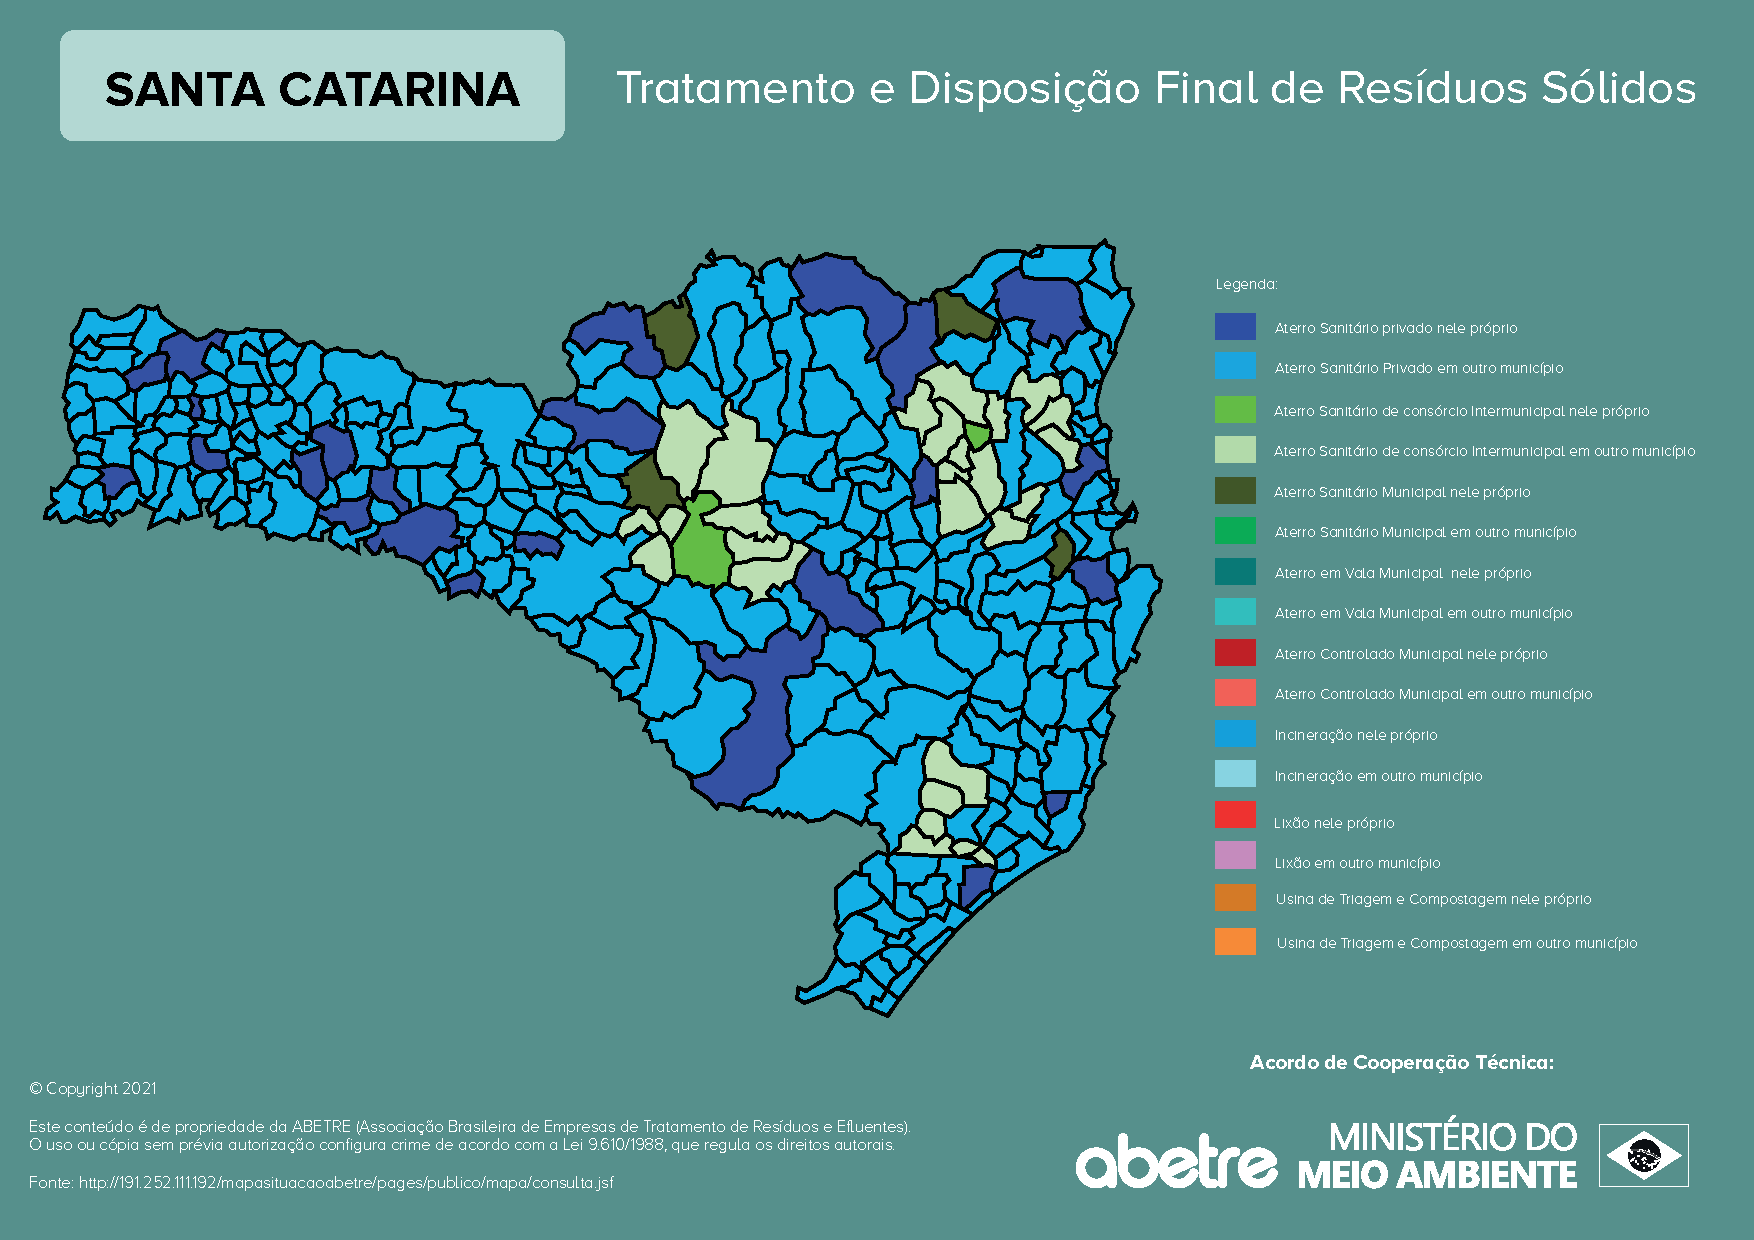
\includegraphics[scale=0.52]{images/abetre_sc.pdf}
	\end{center}
	\fonte{\gls{ABETRE}}
\end{figure}

\pagebreak
% ----------------------------------------------------------
\subsubsection{Aterro}
% ----------------------------------------------------------

Uma das destinações mais comuns no país, são áreas de armazenamento de resíduos \cite{diagnostico_cristine}:
\begin{itemize} 
	\item \textbf{Lixão:} a céu aberto;
	\item \textbf{Aterros Controlados:} em locais sem impermeabilização do solo;
	\item \textbf{Aterros Sanitários:} em espaço com engenharia dedicada à maior compactação dos resíduos e menor dano possível ao meio ambiente;
\end{itemize}
% ----------------------------------------------------------
\subsubsection{Tratamentos térmicos}
% ----------------------------------------------------------
Bastante utilizados no ramo da saúde \cite{diagnostico_cristine}:
\begin{itemize} 
	\item \textbf{Autoclave:} consiste na desinfecção dos resíduos através do aquecimento a uma temperatura elevada em contato com o vapor de água superaquecido;
	\item \textbf{Incineração:} queima dos resíduos a temperaturas superiores a 1000 °C numa atmosfera com oxigênio;
	\item \textbf{micro-ondas:} exposição dos resíduos à radiação eletromagnética de alta frequência;
	\item \textbf{Pirólise:} realiza-se o aquecimento dos materiais acima de 1000 °C numa atmosfera sem oxigênio;
\end{itemize}

% ----------------------------------------------------------
\subsubsection{Blendagem e coprocessamento}
% ----------------------------------------------------------

A \textbf{blendagem} é um processo de mistura de resíduos (\textit{"blends"}) a fim de gerar um produto alternativo ou matéria prima. Geralmente são misturados resíduos específicos para substituir ou reduzir o uso de uma matéria prima, barateando o processo. 

O \textbf{coprocessamento} utiliza os \textit{"blends"} de alto poder calorífico para destruição térmica dos resíduos em fornos de cimento resultando numa economia energética e de matéria prima \cite{noauthor_destinacao_nodate}


% ----------------------------------------------------------
\subsubsection{Compostagem}
% ----------------------------------------------------------

Trata-se de um método aeróbio de reciclagem e tratamento de resíduos orgânicos que busca reproduzir as condições observadas no processo natural de degradação da matéria orgânica \cite{diagnostico_cristine}.

% ----------------------------------------------------------
\subsubsection{Descontaminação de lâmpadas}
% ----------------------------------------------------------
Está relacionado à logística reversa das lâmpadas que contém mercúrio em sua composição. Consiste normalmente em pontos de entrega em estabelecimentos comerciais do país. As lampadas coletadas são transportadas e destinadas a recicladores homologados \cite{noauthor_legislacao_2023}.

% ----------------------------------------------------------
\subsubsection{Fins Didáticos}
% ----------------------------------------------------------

Trata da disposição de resíduos para utilização em unidades organizacionais. Por se tratar de uma movimentação de bem móvel entre organizações e órgãos da União fica regido pelo DECRETO Nº 10.340, 2020 \cite{brasil_decreto_2020}

% ----------------------------------------------------------
\subsubsection{Reciclagem} 
% ----------------------------------------------------------
De acordo com a \gls{PNRS}, reciclagem é o “processo de transformação dos resíduos sólidos que não seriam aproveitados, com mudanças em seus estados físico, físico-químico ou biológico, de modo a atribuir características ao resíduo para que ele se torne novamente matéria-prima ou novos produtos [...]” \cite[Art 3º, ítem XIV]{brasil_lei_nodate}.

% ----------------------------------------------------------
\subsubsection{Recuperação Energética}
% ----------------------------------------------------------

A recuperação energética é um processo que utiliza a energia contida nos resíduos sólidos para gerar eletricidade, calor ou combustíveis alternativos através da digestão anaeróbia, recuperação de gás de aterro sanitário, incineração e coprocessamento \cite{abren_abren_2021}

% ----------------------------------------------------------
\subsubsection{Rerrefino} 
% ----------------------------------------------------------

É o processo relacionado a recolhimento, coleta e destinação final de \gls{OLUC} de modo a aproveitar ao máximo seus constituintes e não causar danos ambientais \cite{diagnostico_cristine}.

% ----------------------------------------------------------
\subsubsection{Tratamento de Efluentes}
% ----------------------------------------------------------

Diz respeito à \gls{ETE}, que são: “unidades operacionais do sistema de esgotamento sanitário que através de processos físicos, químicos ou biológicos removem as cargas poluentes do esgoto, devolvendo ao ambiente o produto final,  efluente tratado, em conformidade com os padrões exigidos pela legislação ambiental.” \parencite{casan_ete_2023}

\subsubsection{Uso Agrícola}

É pertinente à utilização de resíduos como fertilizantes, sejam de origem agropecuária, urbana ou industrial. O uso de resíduos como fertilizantes atende requisitos da economia circular, economia verde e resíduo zero. \cite{diagnostico_cristine}


% ----------------------------------------------------------
\section{Classificações de resíduos sólidos industriais}
% ----------------------------------------------------------

A classificação de resíduos sólidos industriais é um processo fundamental que visa identificar suas características, riscos potenciais e formas apropriadas de tratamento e destinação. 

% ----------------------------------------------------------
\subsection{ABNT NBR 10004:2004}
% ----------------------------------------------------------

Para efeitos da norma ABNT NBR 10004:2004 Resíduos Sólidos — Classificação \cite{abnt_abnt_2004}, os resíduos são classificados com base no seu risco ao meio ambiente e à saúde. Os códigos possuem uma letra e três números. A classificação pode ser encontrada no \autoref{qua:Quadro_1}

\begin{quadro}[htb]
	\centering
	\caption{\label{qua:Quadro_1} Classificação de Resíduos Sólidos de acordo com a ABNT NBR 10004:2004}	
	\resizebox{\textwidth}{!}
	{\begin{tabular}{|l|p{11cm}|}
		\hline
		\textbf{Resíduos classe I — Perigosos} & São aqueles que em detrimento das características físicas, químicas e biológicas apresentam riscos a saúde e meio ambiente.  \\ \hline
		\textbf{Resíduos classe II — Não perigosos}        & São resíduos que não apresentam periculosidade aparente, exemplos são: sucatas, madeira, papel e papelão, borracha, areia de fundição, bagaço de cana.\\ \hline
		\textbf{Resíduos classe II A — Não inertes}          & São os resíduos que não se encaixam na classe II B. \\ \hline
		\textbf{Resíduos classe II B — Inertes}        & Quaisquer resíduos que, segundo normas auxiliares (ABNT NBR 10007 e ABNT NBR 10006) não tiverem nenhum de seus constituintes solubilizados e concentrações superiores aos padrões de potabilidade de água, excetuando-se aspecto, cor, turbidez, dureza e sabor. \\ \hline
	\end{tabular}}
	\fonte{\textcite{abnt_abnt_2004}.}
\end{quadro}


% ----------------------------------------------------------
\subsection{CONAMA}
% ----------------------------------------------------------

A RESOLUÇÃO CONAMA nº 358, 2005 \cite{noauthor_legislacao_conama_2005} com vistas a preservar a saúde pública e a qualidade do meio ambiente, dispõe sobre o tratamento e a disposição final dos resíduos dos serviços de saúde e dá outras providências, como a classificação dos resíduos em cinco grupos (A, B, C, D e E), conforme \autoref{qua:Quadro_2}

\begin{quadro}[htb]
	\centering
	\caption{\label{qua:Quadro_2} Classificação de Resíduos Sólidos de acordo com a CONAMA}	
	\resizebox{\textwidth}{!}{\begin{tabular}{|l|p{11cm}|}
		\hline
		\textbf{I — Grupo A} & Resíduos com a possível presença de agentes biológicos que, por suas características de maior virulência ou concentração, podem apresentar risco de infecção.  \\ \hline
		\textbf{II — Grupo B}        & Resíduos contendo substâncias químicas que podem apresentar risco à saúde pública ou ao meio ambiente, dependendo de suas características de inflamabilidade, corrosividade, reatividade e toxicidade\\ \hline
		\textbf{III — Grupo C}          &  Quaisquer materiais resultantes de atividades humanas que contenham radionuclídeos em quantidades superiores aos limites de eliminação especificados nas normas da \gls{CNEN} e para os quais a reutilização é imprópria ou não prevista. \\ \hline
		\textbf{IV — Grupo D}        & Resíduos que não apresentem risco biológico, químico ou radiológico à saúde ou ao meio ambiente, podendo ser equiparados aos resíduos domiciliares. \\ \hline
		\textbf{V — Grupo E}        & Materiais perfurocortantes ou escarificantes, tais como: lâminas de barbear, agulhas, escalpes, ampolas de vidro, brocas, limas endodônticas, pontas diamantadas, lâminas de bisturi, lancetas; tubos capilares micropipetas; lâminas e lamínulas; espátulas; e todos os utensílios de vidro quebrados no laboratório (pipetas, tubos de coleta sanguínea e placas de Petri) e outros similares. \\ \hline
	\end{tabular}}
	\fonte{\textcite{noauthor_legislacao_conama_2005}.}
\end{quadro}

% ----------------------------------------------------------
\subsection{IBAMA}
% ----------------------------------------------------------

O \gls{IBAMA} por meio da INSTRUÇÃO NORMATIVA Nº 13, 2012 \cite{noauthor_instrucao_ibama} define que “A classificação de resíduos sólidos envolve a identificação do processo ou atividade que lhes deu origem, de seus constituintes e características, e a comparação destes constituintes com listagens de resíduos e substâncias cujo impacto à saúde e ao meio ambiente é conhecido.”.

Trata-se da classificação mais completa no Brasil até o momento de publicação desse trabalho, é também a referência para o \gls{MTR}. A estrutura segue um padrão de capítulo, subcapítulo, indicador de periculosidade e resíduo, consolidando no fim o código do resíduo, conforme \autoref{fig:Fig_2}. Atualmente, existe um total de 878 códigos classificando os resíduos sólidos; existe uma lista disponível no \href{https://www.gov.br/ibama/pt-br/assuntos/emissoes-e-residuos/residuos/arquivos?b_start:int=0}{\textbf{site do IBAMA}} nos formatos \href{https://www.gov.br/ibama/pt-br/assuntos/emissoes-e-residuos/residuos/arquivos/ibama-lista-brasileira-de-residuos-solidos.xls/view}{\textbf{.xls}} e \href{https://www.gov.br/ibama/pt-br/assuntos/emissoes-e-residuos/residuos/arquivos/ibama-lista-brasileira-de-residuos-solidos.doc/view}{\textbf{.doc}}

\begin{figure}[h]
	\caption{\label{fig:Fig_2} Exemplo de construção do código de identificação de resíduo do IBAMA}
	\begin{center}
		\includegraphics[scale=0.8]{images/exemplo-codigo-ibama.png}
	\end{center}
	\fonte{\gls{IBAMA}}
\end{figure}


% ----------------------------------------------------------
\section{Principais atividades industriais de SC}
% ----------------------------------------------------------

Para se obter um panorama sobre as atividades industriais que mais contribuem economicamente para o estado foi utilizado a \gls{PIA} - Empresa, o qual é elaborado uma vez por ano pelo \gls{IBGE} e investiga informações sobre as características estruturais básicas do segmento empresarial da atividade industrial no País, tendo como unidade de investigação a empresa industrial formalmente constituída cuja principal fonte de receita seja a atividade industrial \cite{ibge_pia-empresa_2021}. 

A pesquisa realiza o levantamento de diversas informações econômico-financeiras, como: receitas bruta e líquida; valor da transformação industrial; número de empresas e de unidades locais; pessoal ocupado; gastos com pessoal; custos de operação industrial, entre outros aspectos. 

Para os fins deste tópico, considerou-se dados gerais de empresas industriais com 5 ou mais pessoas ocupadas em \gls{SC} em 2021, e no momento o \gls{PIA} abrange apenas os \gls{CNAE} que compreendem as Indústrias Extrativas e Indústrias de Transformação.

Na \autoref{fig:pia_it} é possível observar a predominância da indústria de fabricação de “Produtos alimentícios”, que em conjunto com as indústrias de “Máquinas, aparelhos e materiais elétricos”, “Confecção de artigos de vestuário e acessórios”, “Produtos têxteis”, "Máquinas e Equipamentos” e “Metalurgia” compõem mais de 60\% do \gls{VTI} das Indústrias de Transformação, o restante se divide em diversos outros setores, com destaque para os pontuados no gráfico. 

\begin{figure}[ht]
	\caption{\label{fig:pia_it} VTI por grupo da Indústria de Transformação em SC}
	\begin{center}
		\includegraphics[scale=0.5]{images/pia-ibge-2021-it.png}
	\end{center}
	\fonte{Adaptado das tabelas do \textcite{ibge_pia-empresa_2021}}
\end{figure}

A Indústria Extrativa divide aproximadamente 1,5\% do \gls{VTI} com a Indústria de Transformação, sendo majoritariamente composta pelas indústrias de “Carvão Mineral”, “Pedra, areia e argila” e “Outros minerais não-metálicos”, conforme ilustrado na \autoref{fig:pia_ie}.

\begin{figure}[ht]
	\caption{\label{fig:pia_ie} VTI por grupo da Indústria Extrativa em SC}
	\begin{center}
		\includegraphics[scale=0.6]{images/pia-ibge-2021-ie.png}
	\end{center}
	\fonte{Adaptado das tabelas do \textcite{ibge_pia-empresa_2021}}
\end{figure}

% ----------------------------------------------------------
\section{Coleta de dados sobre resíduos sólidos industriais no Brasil}
% ----------------------------------------------------------

Na Era da Informação, já somos uma sociedade movida a dados, onde as tomadas de decisões são fundamentadas em evidências e informações coletadas por meio de análises e processamento de uma grande quantidade de dados (Big Data) \cite{castells_information_2010}. 

É notável que uma boa gestão de dados permite que tenhamos um melhor entendimento dos processos, e diante disso, reconhece-se a importância da coleta de dados sobre os resíduos sólidos no país para criação de políticas, práticas e ações que promovam o desenvolvimento sustentável, proteção do meio ambiente e melhoria da qualidade de vida da população, sendo um fator imprescindível nos dias atuais na tomada de decisão orientada a dados.

No Brasil, tem-se conhecimento de três principais fontes de dados sobre a geração e destinação de resíduos sólidos, estas são abordadas nas subseções.
% ----------------------------------------------------------
\subsection{MTR}
% ----------------------------------------------------------

Instituído pela portaria Portaria nº 280, de 29 de junho de 2020 \cite{mma_portaria_202}, o \gls{MTR} é uma ferramenta de gestão e documento de declaração nacional de implantação e operacionalização do \gls{PGRS}; a portaria dispõe que:

\begin{citacao}
	A utilização do MTR é obrigatória em todo o território nacional, para todos os geradores de resíduos sujeitos à elaboração de Plano de Gerenciamento de Resíduos Sólidos, conforme disposto no art. 20 da Lei nº 12.305, de 2 de agosto de 2010, que instituiu a Política Nacional de Resíduos Sólidos, como ferramenta online capaz de rastrear a massa de resíduos, controlando a geração, armazenamento temporário, transporte e destinação dos resíduos sólidos no Brasil. \cite[Art. 2º]{mma_portaria_202}
\end{citacao}

É base mais completa em nível de informações de rastreio de resíduos sólidos no âmbito nacional, e utiliza a lista de códigos de resíduos sólidos do \gls{IBAMA} para identificação dos resíduos.

O sistema é englobado ao \gls{SINIR} e requer um cadastro para que os envolvidos possam publicar o \gls{MTR}, sendo possível cadastrar tanto com o \gls{CPF} quanto com o \gls{CNPJ}. Como uma prática estadual estão sendo incorporados ao sistema do \gls{IMA} de cada \gls{UF}, requerendo também um cadastro para prosseguir. Na \autoref{fig:envio-mtr}, ilustra-se a aba de cadastro de manifesto no \href{http://mtr.ima.sc.gov.br/}{\textbf{site de MTR}} do \gls{IMA/SC}.

\begin{figure}[htb]
	\caption{\label{fig:envio-mtr} Janela de cadastro de MTR do IMA/SC }
	\begin{center}
		\includegraphics[scale=0.6]{images/envio-mtr.png}
	\end{center}
	\fonte{Captura de tela gerada pelo Autor (2023)}
\end{figure}

Para efeitos deste trabalho, foram feitas buscas pelos dados nas plataformas de dados abertos do \gls{MMA}, \gls{IBAMA}, \gls{IMA/SC} e do Governo Federal, mas infelizmente os dados não estão acessíveis publicamente até o momento da publicação deste trabalho. Fez-se necessário contactar o \gls{IMA/SC} para solicitação dos dados.



% ----------------------------------------------------------
\subsection{RAPP}
% ----------------------------------------------------------

O \gls{RAPP} faz parte do \gls{CTF/APP}, no qual todas pessoas jurídicas cadastradas, isolada ou cumulativamente, nas atividades constantes dos da Lei 6.938/1981 para as quais é obrigatório o preenchimento do formulário do \gls{RAPP}, conforme expresso nos Anexos I a XXVI da Instrução Normativa IBAMA n°06/2014. 

O relatório apresenta a relação de geradores de resíduos sólidos por Município/UF e por atividade cadastrada, descrição do resíduo gerado, quantidade, ano de geração e classificação de periculosidade. É a base mais completa no que diz respeito à quantidade de dados, contudo a classificação de resíduos é bastante ampla, por ex.: “Resíduos domiciliares”, “Resíduos Industriais”, “Resíduos da Construção Civil”.

Os dados estão acessíveis publicamente na plataforma de dados abertos do \href{https://dadosabertos.ibama.gov.br/organization/ibama?q=res%C3%ADduos&sort=score+desc%2C+metadata_modified+desc}{\textbf{IBAMA}} e também na do \href{https://dados.gov.br/dados/busca?termo=res%25C3%25ADduos%2520s%25C3%25B3lidos}{\textbf{Governo Federal}}.


% ----------------------------------------------------------
\subsection{Programa Nacional Lixão Zero}
% ----------------------------------------------------------


O Programa Nacional Lixão Zero é uma iniciativa da Secretaria de Qualidade Ambiental para implementar a \gls{PNRS}, integrando-se à Agenda Nacional de Qualidade Ambiental Urbana. O objetivo principal é apoiar estados e municípios na gestão adequada dos resíduos sólidos urbanos, com ênfase na disposição final ambientalmente correta. \cite{mma_programa_2019}

O programa dispõe \href{https://www.gov.br/mma/pt-br/acesso-a-informacao/acoes-e-programas/agendaambientalurbana/lixao-zero/Painel}{\textbf{painéis interativos no site}} que permitem a visualização de mapas, gráficos e indicadores relacionados à gestão de resíduos sólidos urbanos e logística reversa. No que tange aos dados, trata-se de uma base bastante completa em termos de informações,identificação dos resíduos e quantidade de dados; já utiliza os códigos de resíduos sólidos do \gls{IBAMA}.


% ----------------------------------------------------------
\subsection{SINIR}
% ----------------------------------------------------------

O \gls{SINIR} é um instrumento da \gls{PNRS} sob a responsabilidade do Governo Federal, por meio do \gls{MMA}. Com objetivo de unificar os dados sobre resíduos sólidos provenientes de diversas fontes, como o \gls{MTR}, \gls{RAPP}, \gls{SNIS}, \gls{IBGE}. No intuito de criar uma visualização integrada dessas bases o \gls{SINIR}+ compõe uma plataforma tecnológica para apoio à formulação de políticas públicas, em nível nacional, estadual e municipal, permitindo a gestão continuada de resíduos sólidos, além da criação de estratégias e oportunidades de negócios \cite{sinir_sinir_nodate}.

A plataforma é composta de mapas, painéis e relatórios que sistematizam os dados das fontes envolvidas e disponibilizam estatísticas e indicadores referentes à gestão de resíduos sólidos no Brasil. Apesar da plataforma do \gls{SINIR}+ integrar os dados em mapas e relatórios, e conforme mencionado no site que “[...] Professores e estudantes podem navegar em busca de informações gerais sobre os territórios em estudo, comparando regiões e entendendo os diferentes modelos de gestão empregados [...]” não foram encontrados arquivos de dados abertos em formatos que possibilitam uma análise mais específica da situação, por exemplo em \gls{CSV} ou \gls{JSON}.

A \autoref{fig:sinir-mapa} ilustra a visualização de mapa interativo disponibilizado pelo \gls{SINIR}+ que permite a aplicação de camadas sob o mapa, permitindo visualizar correlações entre a geração/destinação de resíduos e infraestrutura urbana, por exemplo.

\begin{figure}[htb]
	\caption{\label{fig:sinir-mapa} Mapa interativo de Gestão de Resíduos Sólidos do SINIR+}
	\begin{center}
		\includegraphics[scale=0.3]{images/sinir-mapa.png}
	\end{center}
	\fonte{Captura de tela gerada pelo Autor (2023)}
\end{figure}

\pagebreak

% ----------------------------------------------------------
\section{Economia Circular}
% ----------------------------------------------------------
A economia circular é um conceito que visa transformar o modelo econômico tradicional linear, baseado na extração, produção, consumo e descarte, em um modelo mais sustentável, que permita repensar as práticas econômicas da sociedade atual e que se inspira no funcionamento da própria Natureza \cite{leitao_economia_2015}. Neste quadro de desenvolvimento, os produtos possuem um ciclo fechado, protegendo e provendo ao meio ambiente, enquanto trabalha em paralelo com a intenção de compra e valor de mercado.

Neste cenário, englobando o pensamento de berço-a-berço (\textit{“Cradle to Cradle”}) \cite{braungart_cradle_2009}, há a oportunidade de fomentar o surgimento de novas dinâmicas entre as empresas, que passam de geradoras de resíduos numa cadeia produtiva, para consumidoras e fornecedoras de materiais num ciclo produtivo. 


% ----------------------------------------------------------
\section{Estado da arte}
% ----------------------------------------------------------

No contexto do gerenciamento de resíduos, existem muitos produtos surgindo para sanar uma lacuna no mercado e auxiliar empresas a melhorar a gestão da informação. Podemos citar os sistemas de gerenciamento “\href{https://www.meuresiduo.com/}{\textbf{meuResíduo}}” e “\href{https://www.resitrack.com.br/}{\textbf{Resitrack}}”, que com propostas bastante semelhantes permitem a unificação do controle de resíduos em um só lugar, substituindo as plataformas do Governo por uma ferramenta mais completa, que automatiza todo o processo de gestão da geração, armazenamento, transporte e destinação integrando com o sistema de \gls{MTR}.

No que diz respeito a uma plataforma de reinserção ou redirecionamento de resíduos no ciclo produtivo, podemos mencionar a “\href{https://www.cataki.org/}{\textbf{Cataki}}”, “\href{https://www.instagram.com/reciclae/}{\textbf{Reciclaê}}” e “\href{https://www1.sfiec.org.br/fiec-noticias/search/134129/sindiverde-lanca-app-que-conecta-produtores-de-residuos-a-industrias-de-reciclagem}{\textbf{Coleta Verde}}”, todos conectando a pessoas ou empresas geradoras a indústrias de reciclagem associadas. Ainda nesse âmbito, podemos mencionar a startup “\href{https://www.urupe.eco.br/}{\textbf{urupê}}”, que com uma proposta de gestão e consultoria realiza todo o processo relacionado a resíduos, visando garantir o maior aproveitamento dos resíduos.

Outra proposta, é a “\href{https://www.bubuyog.com.br/}{\textbf{bubuyog}}”, autonomeada \textit{“Tinder do Aço”}, que com uma plataforma estilo “\textit{marketplace}” auxilia as indústrias do ramo de aço a venderem produtos que, por algum motivo, ficaram parados nos estoques.
% ---

% ---
% 3 - Capítulo 3
% ---
% ----------------------------------------------------------
\chapter{METODOLOGIA}
% ----------------------------------------------------------

% ----------------------------------------------------------
\section{Fontes de dados}\label{section:Fontes}
% ----------------------------------------------------------

Para este trabalho foram utilizados marjoritariamente dados acessíveis publicamente, com exceção aos dados de \gls{MTR}, que foi necessário solicitar ao \gls{IMA/SC}

\subsection{MTR}

Decidiu-se utilizar a base de MTR, pois se trata do banco mais completo em termos de informações, além de que se entende que a mesma será o futuro do rastreamento de resíduos sólidos no país.

Os dados de geração de resíduos sólidos em \gls{SC} de 2020 a 2021 foram extraídos de relatórios em \gls{PDF} fornecidos pelo \gls{IMA/SC}. Infelizmente os dados foram gerados de maneira agrupada, isto é, no total dos dois anos.

\subsection{IBGE}

Com o objetivo de obter os dados relativos a nome de município e coordenadas geográficas foram utilizados os dados abertos mais recentes (2023) de munícipios e de malhas geográficas do \gls{IBGE}. Ambos disponíveis na \href{https://servicodados.ibge.gov.br/api/docs/}{\textbf{\gls{API} de serviço de dados}} do instituto.

\subsection{Portal de Dados Abertos}

Para extrair informações relativas a endereço, situação cadastral, \gls{CNAE} e telefone das empresas foram utilizados os dados mais recentes (2022) de \gls{CNPJ} disponíveis no \href{https://dados.gov.br/dados/conjuntos-dados/cadastro-nacional-da-pessoa-juridica---cnpj}{\textbf{Portal de Dados Abertos do Governo Federal.}}

% ----------------------------------------------------------
\section{Extração, processamento, armazenamento e análise de dados}
% ----------------------------------------------------------

A extração dos dados dos relatórios de \gls{MTR} gerados pelo \gls{IMA/SC} foi feita utilizando a linguagem de programação \href{https://www.python.org/}{\textbf{Python}}. Foram 13 relatórios contendo no total 294 páginas, das quais os dados foram extraídos utilizando as bibliotecas \href{https://tabula.technology/}{\textbf{tabula}} e \href{https://pymupdf.readthedocs.io/en/latest/}{\textbf{Fitz-PyMuPDF}}.

Os dados de municípios e coordenadas geográficas foram extraídos através de requisições \gls{HTTP} direcionadas aos \gls{URI} das \gls{API}s disponibilizadas pelo \href{https://servicodados.ibge.gov.br/api/docs/}{\textbf{\gls{API} de serviço de dados}} do \gls{IBGE} utilizando a biblioteca \href{https://pypi.org/project/requests/}{\textbf{requests}}.

Já a extração dos dados de \gls{CNPJ}, devido a oferta desses dados serem escondidos atrás de \gls{CAPTCHA} ou segregados em arquivos \gls{CSV}, torna-se bastante onerosa a consulta e carregamento dos dados, por isso foi utilizada a \gls{API} \href{https://docs.minhareceita.org/}{\textbf{MinhaReceita}}, que realizou a união de todos os arquivos e os disponibilizou de maneira acessível e gratuita através de requisições \gls{HTTP}; possibilitou-se então, utilizar a biblioteca \href{https://pypi.org/project/requests/}{\textbf{requests}} para requisitar ao \gls{URI}.

Todo processamento dos dados foi feito em máquina pessoal com Processador Intel I7 (8 núcleos), 16GB de \gls{RAM} e disco \gls{SSD}; não foi necessária a utilização de \textit{frameworks} de processamento de dados.

O armazenamento foi feito em máquina virtual disponível em núvem (\textit{Cloud Computing}) utilizando o banco de dados estruturado \href{https://www.postgresql.org/}{\textbf{PostgreSQL}}.

A limpeza e análise dos dados foi feita utilizando a biblioteca \href{https://pandas.pydata.org/}{\textbf{Pandas}} e \gls{SQL}.

Os cálculos relativo a rotas e distâncias entre cidades foram feitos utilizando o serviço gratuito {https://openrouteservice.org/}{\textbf{openrouteservice}}. A criação de de mapas foi feita utilizando as bibliotecas \href{https://pypi.org/project/folium/}{\textbf{Folium}} e \href{https://geopandas.org/en/stable/}{\textbf{Geopandas}}

% ----------------------------------------------------------
\section{Desenvolvimento web}
% ----------------------------------------------------------

O desenvolvimento do aplicativo web foi feito utilizando \href{https://www.python.org/}{\textbf{Python}} com o \textit{framework} \href{https://www.djangoproject.com/}{\textbf{Django}} para a lógica de servidor (“\textit{back-end}”) e \gls{HTML}, \gls{CSS} junto à biblioteca \href{https://htmx.org/}{\textbf{HTMX}} para a interface gráfica (“\textit{front-end}”).

A plataforma foi hospedada em servidor na núvem numa máquina de 4GB de \gls{RAM}, 80 GB de \gls{SSD} e processador Intel com 2 núcleos virtuais. A provedora escolhida foi a \href{https://www.digitalocean.com/}{\textbf{DigitalOcean}}, motivando-se pelo custo fixo e crédito estudantil de 200 dólares via \href{https://education.github.com/pack}{\textbf{GitHub Pro (benefício cedido a estudantes da UFSC)}}, suficiente para manter a máquina ligada por cerca de 6 meses.

Também foram utilizadas as melhores práticas de versionamento de código com \href{https://git-scm.com/}{\textbf{Git}}, containerização com \href{https://www.docker.com/}{\textbf{Docker}}, balanceamento de carga e proxy com \href{https://www.nginx.com/}{\textbf{NGINX}} e certificação \gls{SSL}. Todas tecnologias gratuitas.
% ---

% ---
% 4 - Capítulo 4
% ---
% ----------------------------------------------------------
\chapter{Desenvolvimento}
% ----------------------------------------------------------

As conclusões devem responder às questões da pesquisa, em relação aos objetivos e às hipóteses. Devem ser breves, podendo apresentar recomendações e sugestões para trabalhos futuros.

% ----------------------------------------------------------
\section{Análise exploratória dos dados de MTR}
% ----------------------------------------------------------

% ----------------------------------------------------------
\subsection{Geração}
% ----------------------------------------------------------

% ----------------------------------------------------------
\subsection{Destinação}
% ----------------------------------------------------------

% ----------------------------------------------------------
\subsection{Anomalias e/ou erros de coleta}
% ----------------------------------------------------------

% ----------------------------------------------------------
\subsection{Filtros aplicados}
% ----------------------------------------------------------

% ----------------------------------------------------------
\section{Potenciais usuários consumidores}
% ----------------------------------------------------------

% ----------------------------------------------------------
\section{Levantamento de métricas para o match}
% ----------------------------------------------------------

% ----------------------------------------------------------
\subsection{Quantidade}
% ----------------------------------------------------------

% ----------------------------------------------------------
\subsection{Distância}
% ----------------------------------------------------------

% ----------------------------------------------------------
\subsection{Constância}
% ----------------------------------------------------------

% ----------------------------------------------------------
\subsection{Composição química}
% ----------------------------------------------------------

% ----------------------------------------------------------
\subsection{Cálculo da pontuação}
% ----------------------------------------------------------

% ----------------------------------------------------------
\section{Aplicativo web}
% ----------------------------------------------------------

% ----------------------------------------------------------
\subsection{Conceito I}
% ----------------------------------------------------------

% ----------------------------------------------------------
\subsection{Conceito II}
% ----------------------------------------------------------

% ----------------------------------------------------------
\subsection{Fluxo do usuário}
% ----------------------------------------------------------

% ----------------------------------------------------------
\subsection{Uso de dados}
% ----------------------------------------------------------

% ----------------------------------------------------------
\subsection{Protótipo}
% ----------------------------------------------------------

% ----------------------------------------------------------
\subsubsection{Limitações}
% ----------------------------------------------------------

% ----------------------------------------------------------
\subsubsection{Possíveis adições e melhorias}
% ----------------------------------------------------------
% ---

% ---
% 5 - Conclusão
% ---
%\phantompart
% ----------------------------------------------------------
\chapter{Conclusão}
% ----------------------------------------------------------

No decorrer deste trabalho, entendeu-se que nos últimos 10 anos o poder público investiu em instrumentos que coletam informações sobre resíduos industriais, como o \gls{RAPP}, o Inventário de Resíduos Sólidos Industriais, as Declarações Anuais de Resíduos Sólidos, o programa Lixão Zero, o desenvolvimento do \gls{SINIR} com intuito de agregar todos esses dados, e então o sistema \gls{MTR}. 

Diante disso, a concepção de um produto voltado ao aproveitamento de resíduos sólidos possui inúmeros desafios, pois para alcançar às necessidades de um mercado cada vez mais acelerado as informações devem estar claras, breves e concisas. Nesse sentido, a adoção do \gls{MTR} como base para o sistema aqui discutido prevê que maiores esforços sejam colocados pelos governos estaduais para a disseminação do preenchimento responsável dos manifestos, a acessibilidade dos dados para todos e o estímulo ao empreendedorismo dentro deste mercado.

A proposta do aplicativo web, nomeado “Residuose”, abrangiu dois conceitos, o primeiro para se ter um protótipo funcional disponível para conhecer as dificuldades relacionadas a construção de um sistema desse tipo. Já o segundo foi o resultado do amadurecimento de ideias e expectativas anteriores ao desenvolvimento, considerando-se como uma próxima etapa, mas que ainda depende de maior disponibilidade de acesso aos dados de \gls{MTR}, recursos financeiros, pessoas capacitadas e tempo para o trabalho. De qualquer forma, viu-se através da análise dos dados a existência de uma preocupação notável em \gls{SC} com a destinação dos resíduos, o que é um indicativo de quê um sistema facilitador e incremental às indústrias seja bem-vindo. Para futuros trabalhos, sugere-se:
\begin{itemize} 
	\item A elaboração de pesquisas direcionadas à caracterização de resíduos sólidos de acordo com as classificações do \gls{IBAMA}, para que se tenham maiores informações sobre o material, tornando-o mais visível para empresas interessadas;
	\item O estudo da utilização de \gls{LLM}s no âmbito da Ciência de Materiais para o levantamento, através de artigos acadêmicos, dos potenciais resíduos substitutos de matérias-primas na indústria e como eles se relacionam com as classificações existentes de \gls{RSI}s; 
	\item A busca por fundos de fomento ao empreendedorismo acadêmico para que o projeto tenha recursos, orientação empresarial, levando à capacidade de crescimento das pessoas envolvidas e do produto;
	\item Um melhor alinhamento com o \gls{IMA/SC} para obtenção de dados numa menor granularidade e com maior riqueza de informações;
	\item Um estudo de caso de uma combinação entre duas empresas para que o aplicativo lide com uma situação real revelando problemáticas não abordadas neste documento.
\end{itemize}
% ---


% ----------------------------------------------------------
% ELEMENTOS PÓS-TEXTUAIS
% ----------------------------------------------------------
\postextual
% ----------------------------------------------------------

% ----------------------------------------------------------
% Referências bibliográficas
% ----------------------------------------------------------

\begingroup
    \SingleSpacing\printbibliography[title=REFERÊNCIAS]
\endgroup

% ----------------------------------------------------------
% Glossário
% ----------------------------------------------------------
%
% Consulte o manual da classe abntex2 para orientações sobre o glossário.
%
%\glossary

% ----------------------------------------------------------
% Apêndices
% ----------------------------------------------------------

% ---
% Inicia os apêndices
% ---
% \begin{apendicesenv}
% %	\partapendices* 
% 	\input{aftertext/apendice_a}
% \end{apendicesenv}
% ---


% ----------------------------------------------------------
% Anexos
% ----------------------------------------------------------

% ---
% Inicia os anexos
% ---
% \renewcommand{\appendixautorefname}{Anexo}
\begin{anexosenv}
	% \partanexos*
	% ----------------------------------------------------------
\chapter{Classificação de Resíduos Sólidos por Capítulos do IBAMA}\label{cap:anexo-a}
% ----------------------------------------------------------

De acordo com a a Instrução Normativa nº 13 do \textcite{noauthor_instrucao_ibama}

% Define a new column type for centered text with specified width
\newcolumntype{C}[1]{>{\arraybackslash}m{#1}}

\begin{table}[htb]
    \ABNTEXfontereduzida
    \centering
    \caption{Classificação de Resíduos Sólidos por Capítulos do IBAMA \label{tab:tab-cap-ibama} }
    \begin{tabular}{@{}c C{0.85\linewidth}@{}}
        \toprule
        \textbf{Capítulo} & \textbf{Descrição}                                                                                                                  \\ \midrule
        1                 & Resíduos da prospecção e exploração de minas e pedreiras, bem como de tratamentos físicos e químicos das matérias extraídas         \\
        2 &
          Resíduos da agricultura, horticultura, aquicultura, silvicultura, caça e pesca, e da preparação e processamento de produtos alimentares \\
        3                 & Resíduos do processamento de madeira e da fabricação de painéis, mobiliário, papel e celulose                                       \\
        4                 & Resíduos da indústria do couro e produtos de couro e da indústria têxtil                                                            \\
        5                 & Resíduos da refinação de petróleo, da purificação de gás natural e do tratamento pirolítico do carvão                               \\
        6                 & Resíduos de processos químicos inorgânicos                                                                                          \\
        7                 & Resíduos de processos químicos orgânicos                                                                                            \\
        8 &
          Resíduos da fabricação, formulação, distribuição e utilização de revestimentos (tintas,  vernizes e esmaltes vítreos), colas, vedantes e tintas de impressão \\
        9                 & Resíduos da indústria fotográfica                                                                                                   \\
        10                & Resíduos de processos térmicos                                                                                                      \\
        11                & Resíduos de tratamentos químicos e revestimentos de metais e outros materiais; resíduos da hidrometalurgia de metais não ferrosos   \\
        12                & Resíduos da moldagem e do tratamento físico e mecânico de superfície de metais e plásticos                                          \\
        13                & Óleos usados e resíduos de combustíveis líquidos (exceto óleos alimentares e capítulos 05, 12 e 19)                                 \\
        14                & Resíduos de solventes, fluidos de refrigeração e gases propulsores orgânicos (exceto 07 e 08)                                       \\
        15                & Resíduos de embalagens; absorventes, panos de limpeza, materiais filtrantes e vestuário de proteção não anteriormente especificados \\
        16                & Resíduos não especificados em outros capítulos desta Lista                                                                          \\
        17                & Resíduos de construção e demolição (incluindo solos escavados de locais contaminados)                                               \\
        18                & Resíduos dos serviços de saúde                                                                                                      \\
        19 &
          Resíduos de instalações de gestão de resíduos, de estações de tratamento de águas  residuais e da preparação de água para consumo humano e água para consumo industrial \\
        20 &
          Resíduos sólidos urbanos e equiparados (resíduos domésticos, do comércio, indústria e serviços), incluindo as frações provenientes da coleta seletiva \\ \bottomrule
        \end{tabular}
    \fonte{Elaborado pelo Autor, de acordo com o \textcite{noauthor_instrucao_ibama}}
    \end{table}
\end{anexosenv}

%---------------------------------------------------------------------
% INDICE REMISSIVO
%---------------------------------------------------------------------
%\phantompart
%\printindex
%---------------------------------------------------------------------

\end{document}
